
本章的其餘部分中,將更詳細地瞭解每種性能分析工具。本節中,我們將做一個端到端示例,並分析程序的性能。並展示如何進行性能分析,以及如何使用不同的性能分析工具。

本節結束時,讀者們應該會相信\textit{永遠不要對性能進行猜測}。

實際中需要分析和優化的程序很可能大到要用很篇幅來說明,因此我們將使用一個簡化的示例。程序中將完成對子字符串的排序:假設有一個字符串\texttt{S},比如:\texttt{abcdcba}(這裡是個簡單的例子,實際的字符串可能有數百萬個字符)。可以以該字符串中的任何字符開始創建子字符串,例如:\texttt{S0}的起始偏移量為0,因此其值為\texttt{abcdcba}。\texttt{S2}以偏移量2開始,值為\texttt{cdcba},S5為\texttt{ba}。我們要用常規的字符串比較來按順序對這些子字符串進行排序,子字符串的順序是\texttt{S2},\texttt{S5},\texttt{S0}(按照第一個字符\texttt{'c'}、\texttt{'b'}和\texttt{'a'}的順序)。

如果用字符指針表示子字符串,就可以使用STL的\texttt{std::sort}進行排序。現在交換兩個子字符串只需要交換指針,字符串保持不變。下面是示例代碼:

%\hspace*{\fill} \\ %插入空行
\noindent
\textbf{01\_substring\_sort.C}
\begin{lstlisting}[style=styleCXX]
bool compare(const char* s1, const char* s2, unsigned int l);
int main() {
	constexpr unsigned int L = …, N = …;
	unique_ptr<char[]> s(new char[L]);
	vector<const char*> vs(N);
	  … prepare the string …
	size_t count = 0;
	system_clock::time_point t1 = system_clock::now();
	std::sort(vs.begin(), vs.end(),
	  [&](const char* a, const char* b) {
		++count;
		return compare(a, b, L);
	});
	system_clock::time_point t2 = system_clock::now();
	cout << "Sort time: " <<
	  duration_cast<milliseconds>(t2 - t1).count() <<
	  "ms (" << count << " comparisons)" << endl;
}
\end{lstlisting}

注意,為了編譯這個例子,需要包含相應的頭文件,並使用\texttt{using}聲明一些縮寫:

\begin{lstlisting}[style=styleCXX]
#include <algorithm>
#include <chrono>
#include <cstdlib>
#include <cstring>
#include <iostream>
#include <memory>
#include <random>
#include <vector>
using std::chrono::duration_cast;
using std::chrono::milliseconds;
using std::chrono::system_clock;
using std::cout;
using std::endl;
using std::minstd_rand;
using std::unique_ptr;
using std::vector;
\end{lstlisting}

後面的例子中,將省略公共頭文件和公共名稱(如\texttt{cout}或\texttt{vector})的\texttt{using}聲明。

示例定義了一個字符串,該字符串用於要排序的子字符串和子字符串組(字符指針)的數據(但這裡還沒有展示數據是如何創建的)。然後,使用\texttt{std::sort}和比較函數對子字符串進行排序,調用比較函數\texttt{compare()}的Lambda表達式。我們使用Lambda表達式將\texttt{compare()}函數的輸入(該函數接受兩個指針和最大字符串長度)調整為\texttt{std::sort}所期望的輸入(只有兩個指針),這就是\textbf{適配器模式}。

我們的例子中,Lambda表達式的第二個作用是,用於計算比較調用的次數。因為我們對排序的性能很感興趣,所以如果想比較不同的排序算法,這個信息會很有用(我們現在不打算這麼做,但是這個對讀者們的性能優化工作很有用)。

這個例子中只聲明瞭比較函數,但沒有定義。它的定義在一個單獨的文件中,如下所示:


%\hspace*{\fill} \\ %插入空行
\noindent
\textbf{01\_substring\_sort\_a.C}
\begin{lstlisting}[style=styleCXX]
bool compare(const char* s1, const char* s2, unsigned int l) {
	if (s1 == s2) return false;
	for (unsigned int i1 = 0, i2 = 0; i1 < l; ++i1, ++i2) {
		if (s1[i1] != s2[i2]) return s1[i1] > s2[i2];
	}
	return false;
}
\end{lstlisting}

兩個字符串的簡單比較。如果第一個字符串大於第二個字符串,則返回true,否則返回false。我們可以將函數定義在與代碼相同的文件中,在這個小示例中,我們也會嘗試模擬真實程序的行為,該程序可能會使用分佈在許多不同文件中的函數。因此,本章的\texttt{compare.C}文件中的實現了比較函數,其餘的例子在\texttt{example.C}文件中。

最後,使用\texttt{chrono}庫中的高精度計時器來測量,統計子字符串排序所需的時間。

示例中缺少字符串的實際數據。子字符串排序在許多應用程序中是一項常見的任務,並且每個應用程序都有自己獲取數據的方法。我們的例子中,可以使用生成的隨機字符串。另一方面,在許多子字符串排序的實際應用中,會有一個字符在字符串中出現的頻率比其他任何字符都要高。

我們也可以模擬這種類型的數據,用一個字符填充字符串,然後隨機改變其中的一些字符:

%\hspace*{\fill} \\ %插入空行
\noindent
\textbf{01\_substring\_sort\_a.C}
\begin{lstlisting}[style=styleCXX]
constexpr unsigned int L = 1 << 18, N = 1 << 14;
unique_ptr<char[]> s(new char[L]);
vector<const char*> vs(N);
minstd_rand rgen;
::memset(s.get(), 'a', N*sizeof(char));
for (unsigned int i = 0; i < L/1024; ++i) {
	s[rgen() % (L - 1)] = 'a' + (rgen() % ('z' - 'a' + 1));
}
s[L-1] = 0;
for (unsigned int i = 0; i < N; ++i) {
	vs[i] = &s[rgen() % (L - 1)];
}
\end{lstlisting}

字符串的長度\texttt{L}和子字符串的數量\texttt{N}運行的時長,需要適配相應的硬件(如果想在其他設備上重複運行這個例子,可能需要調整相應的數字,運行速度速度取決於使用的處理器)。

現在可以編譯和運行了:

%\hspace*{\fill} \\ %插入空行
\begin{center}
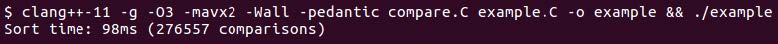
\includegraphics[width=0.9\textwidth]{content/1/chapter2/images/1.jpg}\\
圖 2.1
\end{center}

得到的結果取決於使用的編譯器、運行的硬件環境。當然,還取決於數據的語料庫。

現在我們有了第一個性能測試。現在可能會碰到的第一個問題是,如何優化?嗯……這並不應該是第一個問題。第一個問題應該是,需要優化嗎?要回答這個問題,需要有具體的性能目標和指標,以及這個項目其他部分的性能的數據,例如:如果實際的字符串是由一個耗時10小時的模擬生成的,那麼排序所花費的100秒的時間幾乎可以忽略不計。當然,我們仍是在處理模擬示例,除非我們必須要提高性能,否則本章不會對優化進行討論。

我們準備好討論如何優化它嗎?這個問題先放放。當前的問題應該是,\textbf{應該優化什麼}?或者說,程序在什麼地方花費的時間最多?即使在這個例子中,這個耗時熱點可能是排序,或是比較函數。對於不能訪問的源碼(除非想破壞標準庫),可以將計時器放入到相應的函數前後。

不過,這不太可能產生好的結果。因為調用計時器也需要時間,所以每次調用比較函數時,若每次運行比較都非常快,調用計時器的時間將對測試結果有較大的影響。實際的程序中,這種帶有計時器的結構幾乎沒有。如果不知道時間耗費在哪裡,就需要在數百個函數中安插計時器(如果沒有測試,要如何知道這一點?)。所以,這時就需要性能分析工具來幫助我們來完成一些工作了。

下一節中會介紹更多關於分析器的知識。現在,只需瞭解以下命令行將編譯和執行的程序,並使用GperfTools包中的谷歌分析器,收集其運行時的相關信息即可:

%\hspace*{\fill} \\ %插入空行
\begin{center}
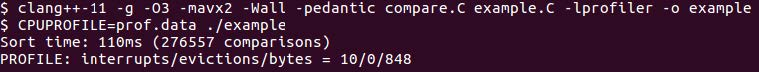
\includegraphics[width=0.9\textwidth]{content/1/chapter2/images/2.jpg}\\
圖 2.2
\end{center}

數據放在\texttt{prof.data}文件中,其路徑由\texttt{CPUPROFILE}環境變量指定。細心的讀者可能已經注意到,這次程序運行的時間更長了,這是性能分析不可避免的副作用。假設分析器本身工作正常,那麼程序不同部分的相對性能仍然是準確的。

輸出的最後一行說明,分析器已經收集了一些數據,現在需要以可讀的格式顯示這些數據。對於谷歌分析器收集的數據,用戶界面工具是\texttt{google-pprof}(通常安裝為簡單的\texttt{pprof}),最簡單的方式是列出程序中的每個函數,以及在該函數中花費時間的百分比(第二列):

%\hspace*{\fill} \\ %插入空行
\begin{center}
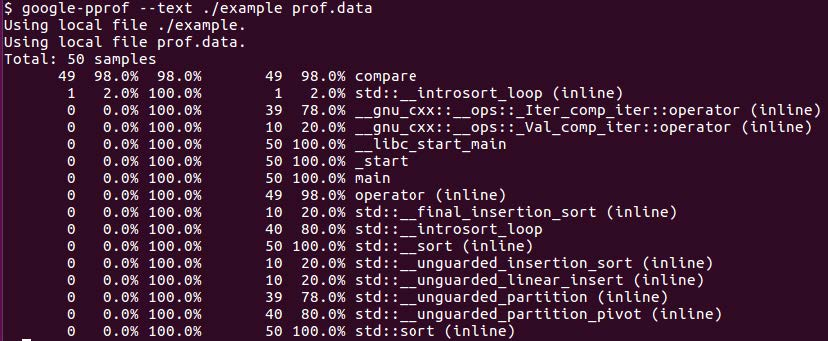
\includegraphics[width=0.9\textwidth]{content/1/chapter2/images/3.jpg}\\
圖 2.3
\end{center}

分析器顯示,大多時間都花在比較函數\texttt{compare()}上,而排序幾乎不花時間(第二行是\texttt{std::sort},應該認為是排序耗時的一部分)。對於任何分析,都需要收集50個以上的樣本數據。樣本數據的數量取決於程序運行的時間,為了獲得可靠的數據,需要在每個要測試的函數中積累至少幾十個樣本數據。就我們的情況而言,其結果比較容易判斷,因此我們會按收集的數據來做分析。

由於子字符串比較函數佔用了總運行時間的98\%,我們只有兩種方法來提高性能:可以使這個函數更快,或者可以減少使用次數(許多人忘記了第二種可能性,直接使用第一種可能性)。第二種方法需要使用不同的排序算法,不在本書的討論範圍之內。這裡我們將重點放在第一個選項上,讓我們再來看一下比較函數的代碼:

%\hspace*{\fill} \\ %插入空行
\noindent
\textbf{01\_substring\_sort\_a.C}
\begin{lstlisting}[style=styleCXX]
bool compare(const char* s1, const char* s2, unsigned int l) {
	if (s1 == s2) return false;
	for (unsigned int i1 = 0, i2 = 0; i1 < l; ++i1, ++i2) {
		if (s1[i1] != s2[i2]) return s1[i1] > s2[i2];
	}
	return false;
}
\end{lstlisting}

這只是幾行代碼,我們應該能夠理解和預測代碼的所有行為。還有一個比較子字符串和它本身的檢查,這肯定比實際逐字符比較要快。所以,除非確定函數調用時兩個指針的值不會相同,否則這一行肯定保持不變。

還有一個循環(循環的主體是一次比較一個字符),這裡必須這樣做,因為不知道哪個字符可能不同。循環本身會一直運行,直到找到一個差值或比較最大可能的字符數為止。顯而易見,後一種情況是不可能發生的:該字符串以空字符結尾,即使兩個子字符串中的所有字符都相同,那也會到達較短子字符串的末尾,將其末尾的空字符與另一個子字符串中的非空字符進行比較,從而確定較短的子字符串是兩者中較短的字符串。

當兩個子字符串都從同一個位置開始時,才有可能讀取字符串末尾以外的內容,所以我們在函數的一開始就進行了檢查。這很好!這裡有了一些不必要的工作,因此可以優化代碼,並避免每次循環迭代都進行一次比較操作(考慮到循環體中沒有很多其他操作)。

代碼中的改動非常簡單,只需刪除循環對長度的比較操作(不再需要將長度傳遞給比較函數):

%\hspace*{\fill} \\ %插入空行
\noindent
\textbf{03\_substring\_sort\_a.C}
\begin{lstlisting}[style=styleCXX]
bool compare(const char* s1, const char* s2) {
	if (s1 == s2) return false;
	for (unsigned int i1 = 0, i2 = 0;; ++i1, ++i2) {
		if (s1[i1] != s2[i2]) return s1[i1] > s2[i2];
	}
	return false;
}
\end{lstlisting}

更少的參數、操作、代碼。運行這個程序,看看這次優化為節省了多少運行時間:

%\hspace*{\fill} \\ %插入空行
\begin{center}
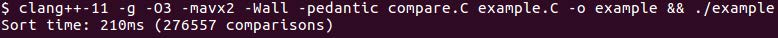
\includegraphics[width=0.9\textwidth]{content/1/chapter2/images/4.jpg}\\
圖 2.4
\end{center}

如果說事情沒有按計劃進行,那就太保守了。原來的代碼花了98毫秒來解決相同的問題(圖2.1)。“優化後的”代碼需要210毫秒,儘管做的工作更少(在這個例子中,並不是所有的編譯器都表現出這種特殊的性能異常,但我們使用的是實際生產過程中使用的編譯器)。

總結一下這個例子,它實際上是一個現實程序的簡單版本。當我們試圖優化這段代碼時,另一個開發者正在使用代碼的另一部分,並且還需要一個子字符串比較函數。將單獨開發的代碼片段放在一起,只保留了這個函數的一個版本,而它恰好是我們沒有修改的那個;其他開發者的修改幾乎同樣:

%\hspace*{\fill} \\ %插入空行
\noindent
\textbf{04\_substring\_sort\_a.C}
\begin{lstlisting}[style=styleCXX]
bool compare(const char* s1, const char* s2) {
	if (s1 == s2) return false;
	for (int i1 = 0, i2 = 0;; ++i1, ++i2) {
		if (s1[i1] != s2[i2]) return s1[i1] > s2[i2];
	}
	return false;
}
\end{lstlisting}

仔細觀察這段代碼和它前面的代碼片段,看看是否能發現區別。

唯一的區別是循環變量的類型。之前,我們使用了\texttt{unsigned int},索引從0開始並向前推進,因為我們不期望有任何負數。後一個代碼片段使用了\texttt{int},放棄了可能的索引值範圍的一半。

對於這個代碼的修改,可以再次運行我們的基準測試,這次是用新的比較函數。結果出人意料:

%\hspace*{\fill} \\ %插入空行
\begin{center}
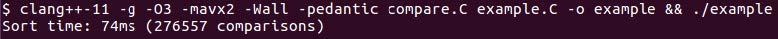
\includegraphics[width=0.9\textwidth]{content/1/chapter2/images/5.jpg}\\
圖 2.5
\end{center}

最新版本耗時74毫秒,比我們最初的版本(98毫秒,圖2.1)快,也比幾乎相同的第二個版本(210毫秒,圖2.2)快得多。

後面的章節中,我們再來解釋這個現象的根本原因。本節的目的是闡明\textbf{永遠不要猜測性能}:“顯而易見”的優化——用更少的代碼做完全相同的計算——反向進行不重要的小改變——使用有符號整數而不是無符號的函數——結果證明是最後一個才是有效的優化。

即使在這個非常簡單的例子中,性能結果也可能與直覺相反。因此,對於性能決策的唯一方法必須是指標驅動。本章的其餘部分,我們將看到一些用於收集性能指標的工具,並將會學習如何使用它們,以及如何解釋其結果。
